% ===== RESULTS
% -- Make all figures relative to this folder
\graphicspath{{./results/}}

\chapter{Results}
\label{sec:Results}

\section
   {Oxygen Dissociation in \ce{O2 + N2} and Aggregate Oxygen Dissociation}
\sectionmark{Oxygen Dissociation in \ce{O2 + N2}}    % -- When header is too big otherwise
\label{sec:O2_N2}
The oxygen dissociation rate with partners \ce{N2}, \ce{O2}, and \ce{O}, for the equilibrium and nonequilibrium test set,
   is shown in \cref{fig:O2-Dissoc_Rates}.
This is a standard side-by-side figure layout for the author.
A standard single-figure layout is \cref{fig:N3_Exchange_Rate}.

% -- Standard two-figure layout
\begin{figure}[p]
   \centering
   \begin{subfigure}[t]{\twofigwidth\textwidth}
      \centering
      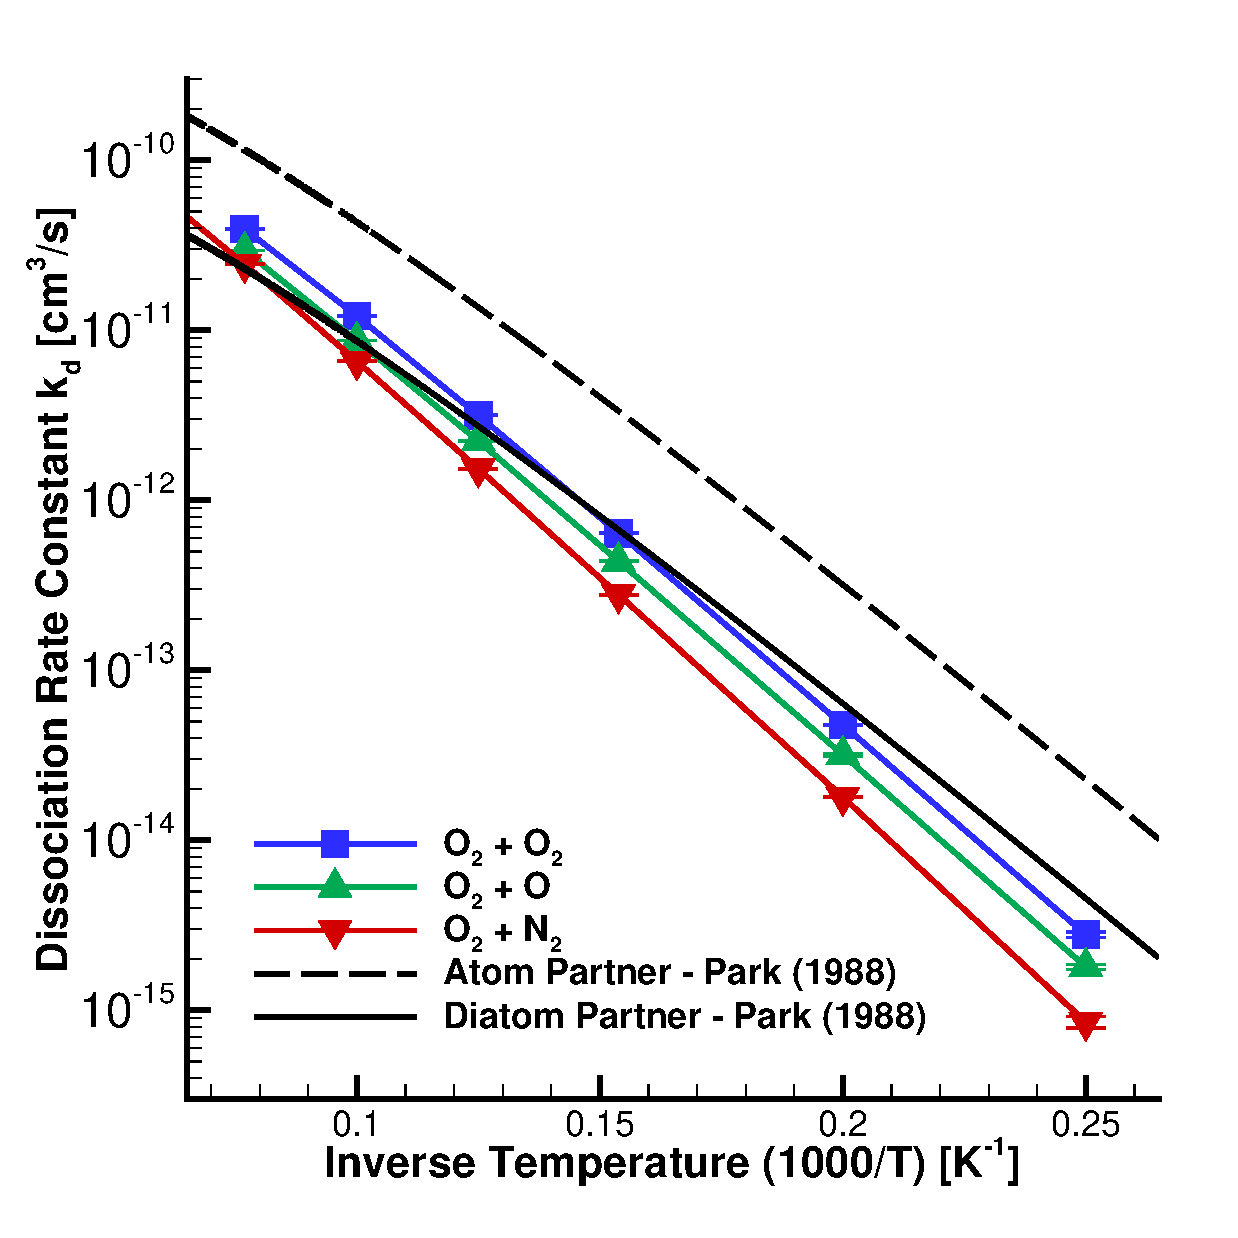
\includegraphics[width=\textwidth]{./figures/O2-Dissoc_AllPartners_Equil.eps}
      \caption{$\Ttr=\Tv$}
   \end{subfigure}
%
   \begin{subfigure}[t]{\twofigwidth\textwidth}
      \centering
      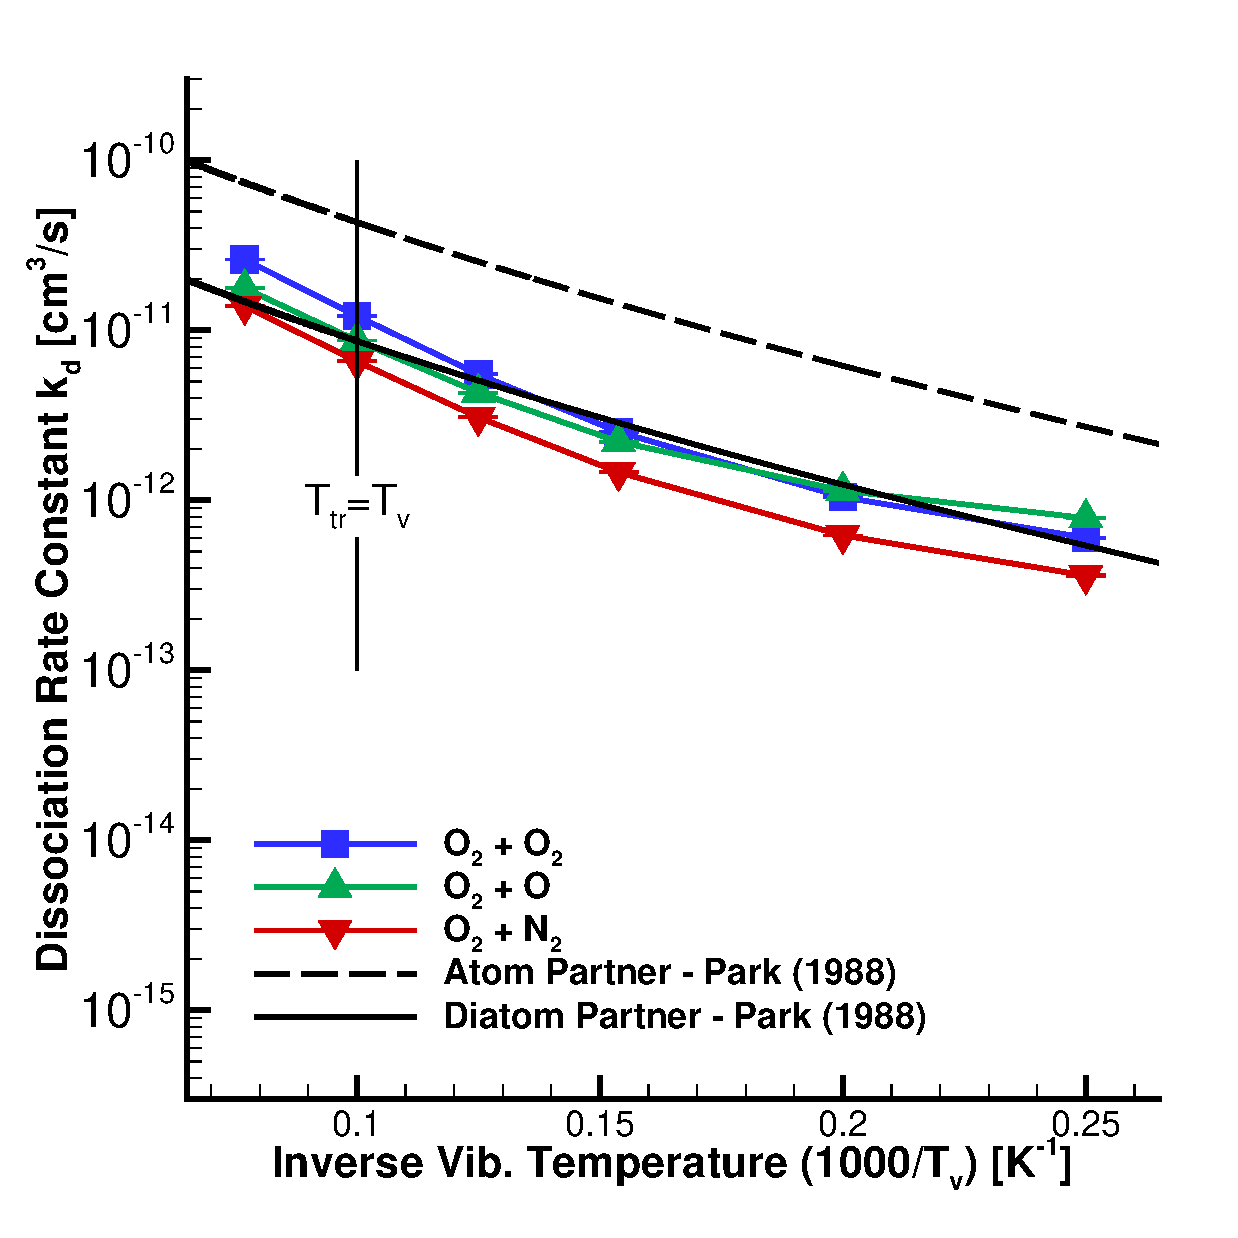
\includegraphics[width=\textwidth]{./figures/O2-Dissoc_AllPartners_Nonequil.eps}
      \caption{$\Ttr=\SI{10000}{\kelvin}$}
   \end{subfigure}
   \caption[Oxygen dissociation with various parameters]
      {Oxygen dissociation rate with collision partners \ce{O2}, \ce{O}, and \ce{N2}
         for the equilibrium and nonequilibrium test set.}
   \label{fig:O2-Dissoc_Rates}
\end{figure}

\begin{figure}[p]
   \centering
   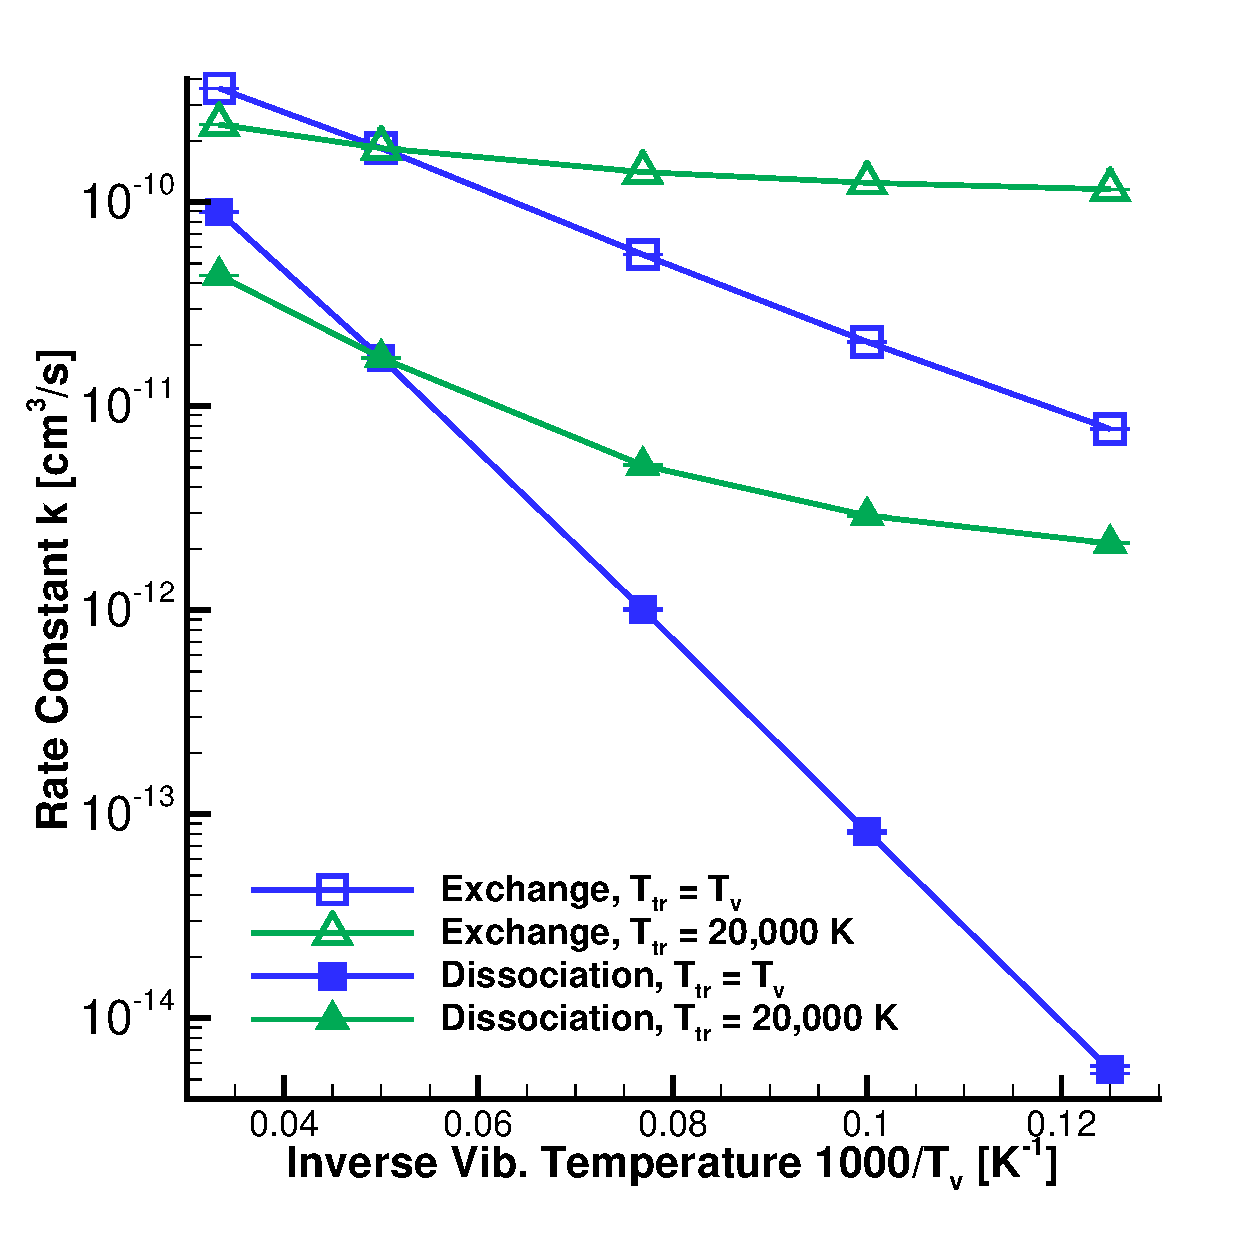
\includegraphics[width=0.48\textwidth]{./figures/N3_Dissoc_vs_Exchange.eps}
   \caption[Exchange and dissociation rates in \ce{N2 + N}]
      {Reaction rate constants for exchange and dissociation in \ce{N2 + N},
      for the equilibrium and nonequilibrium test set.}
   \label{fig:N3_Exchange_Rate}
\end{figure}

For testing, here is a handful of pages filled with junk.
How does the header look, on a page like this?

\lipsum[1-10]
